\documentclass[11pt,a4paper]{article}

\usepackage[utf8]{inputenc}
\usepackage[T1]{fontenc}
\usepackage[spanish,es-nodecimaldot]{babel}
\usepackage[a4paper,margin=2.4cm]{geometry}
\usepackage{amsmath,amssymb}
\usepackage{graphicx}
\usepackage{subcaption}
\usepackage{booktabs}
\usepackage{longtable}
\usepackage{array}
\usepackage{xcolor}
\usepackage{enumitem}
\usepackage[hidelinks]{hyperref}
\usepackage{caption}

\newcommand{\code}[1]{\texttt{\small #1}}
\graphicspath{{figures/}{figures/report/}{figures/cross/}{figures/01_exact/}}

\title{\textbf{Informe Técnico: Experimentos Preliminares sobre SVRPBench}\\[2mm]
\large Comparación homologada de cuatro paradigmas de optimización para el\\
Problema de Enrutamiento de Vehículos Estocástico}
\author{Abraham Castañeda Quintero\\
\small Anteproyecto EHBG-FACS --- Facultad de Ingeniería Mecánica y Eléctrica, UANL}
\date{2026}

\begin{document}
\maketitle

\begin{abstract}
\noindent Este informe documenta la implementación y comparación, bajo condiciones
experimentales \emph{homologadas}, de los cuatro paradigmas clásicos de optimización para
el enrutamiento de vehículos sobre el benchmark estocástico de alta fidelidad
\textbf{SVRPBench}: (1)~métodos exactos (Branch \& Cut), (2)~metaheurísticas (ACO y Tabu),
(3)~optimización combinatoria neuronal (NCO) supervisada (Pointer Networks) y (4)~NCO por
aprendizaje por refuerzo (POMO). Estos cuatro constituyen las líneas base contra las que se
medirá la propuesta de tesis (EHBG-FACS). Se describe la naturaleza del problema, la
generación y las características de las instancias, el modelo estocástico, el marco de
evaluación (programación estocástica en dos etapas con recurso, \emph{Common Random
Numbers}, CVaR) y la homologación de condiciones que garantiza una comparación justa. Los
resultados revelan dos familias bien separadas —métodos de costo óptimo pero frágiles ante
las ventanas de tiempo, frente a métodos factibles pero costosos en flota— y \emph{ningún}
método ocupa la región ideal (bajo costo \emph{y} alta factibilidad), que es precisamente el
hueco que la propuesta busca cerrar. Se incluye un diccionario completo de acrónimos,
variables y métodos.
\end{abstract}

\tableofcontents

% =====================================================================
\section{Naturaleza del problema}
\label{sec:problema}

El \textbf{Problema de Enrutamiento de Vehículos} (VRP) consiste en diseñar un conjunto de
rutas para una flota que parte de un depósito, atiende a un conjunto de clientes
geográficamente distribuidos y regresa al depósito, minimizando el costo total sujeto a
restricciones de capacidad y, en la variante con ventanas de tiempo (TWCVRP), a intervalos
de servicio admisibles por cliente. El VRP es \textbf{NP-duro}: el tiempo para hallar el
óptimo global crece exponencialmente con el número de clientes.

El \textbf{Problema de Enrutamiento de Vehículos Estocástico} (SVRP) reemplaza la idealización
determinista por variables aleatorias: la velocidad de tránsito, los retrasos y las
disrupciones son inciertos. Una ruta óptima en el mundo determinista puede volverse inviable
o muy costosa bajo incertidumbre. Formalmente adoptamos una \textbf{programación estocástica
en dos etapas con recurso}: en la primera etapa se decide la ruta \emph{a priori} (antes de
observar el escenario aleatorio $\xi$); en la segunda, cuando la ruta resulta inviable (p.\,ej.\
una ventana violada), se aplica una política de recurso con costo $Q(\text{ruta},\xi)$. El
costo total de una solución es $c(\text{ruta}) + Q(\text{ruta},\xi)$, estimado por simulación
Monte Carlo.

% =====================================================================
\section{El benchmark SVRPBench y las instancias}
\label{sec:bench}

\subsection{Naturaleza de las instancias}

Las instancias se generan reutilizando las primitivas oficiales de SVRPBench
(\code{city.City.batch\_sample} para las ubicaciones y
\code{time\_windows\_generator.sample\_time\_window} para las ventanas). Cada instancia de
$n$ clientes (más un depósito único) tiene:
\begin{itemize}[nosep]
  \item \textbf{Ubicaciones} agrupadas: los clientes se muestrean de una distribución normal
  alrededor de un centro de ciudad sobre un mapa de $1000\times1000$ unidades; el depósito se
  sitúa en el centroide de los clientes (Fig.~\ref{fig:instance}).
  \item \textbf{Demandas} enteras $\sim \mathcal{U}[1,100]$ (se usa $1$ como cota inferior, no
  la $0$ oficial, para que el único nodo de demanda nula sea el depósito).
  \item \textbf{Ventanas de tiempo} heterogéneas: residenciales (bimodal mañana/tarde) o
  comerciales (alrededor del mediodía).
  \item \textbf{Capacidad restrictiva} $\text{cap}=\max(\text{dem}_{\max},\lceil
  \text{dem}_{\text{total}}/K\rceil)$, de modo que la capacidad sea activa y un CVRP genuino.
\end{itemize}

\begin{figure}[h]
  \centering
  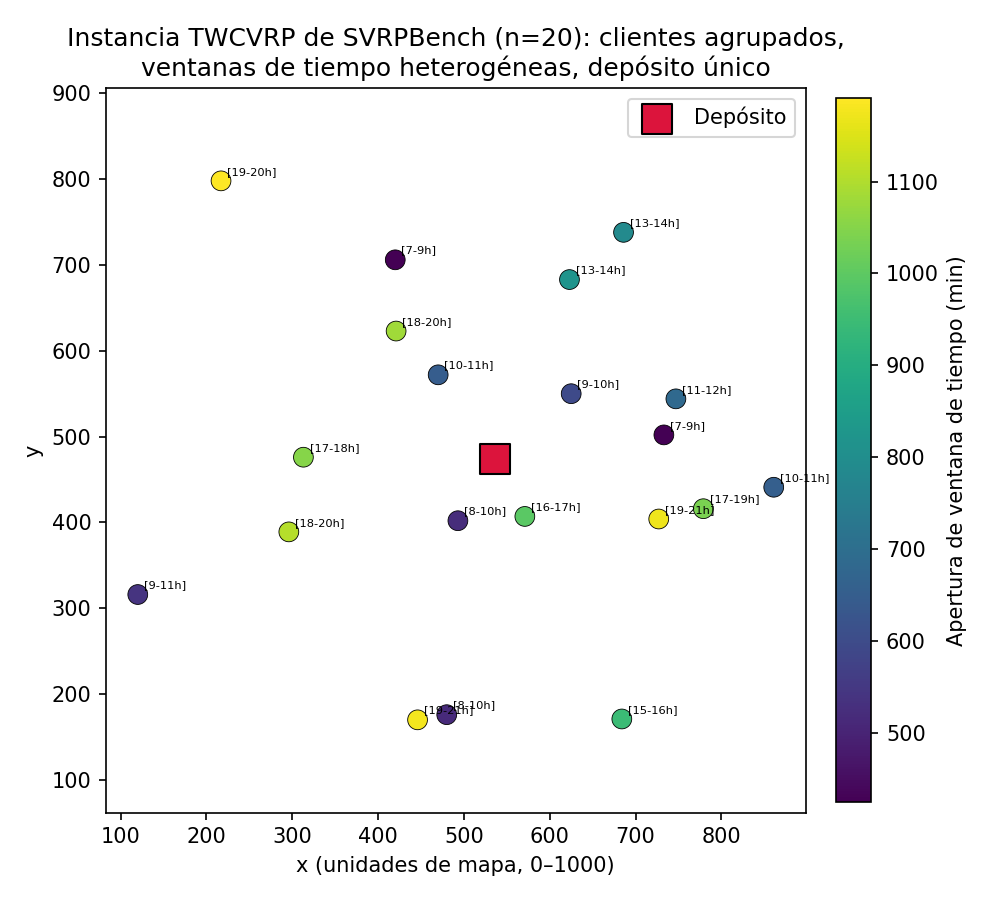
\includegraphics[width=0.62\textwidth]{instance_example.png}
  \caption{Una instancia TWCVRP ($n=20$). El depósito (cuadro rojo) está en el centroide;
  los clientes se colorean por la hora de apertura de su ventana de tiempo; las etiquetas
  indican el intervalo $[\text{apertura}-\text{cierre}]$ en horas.}
  \label{fig:instance}
\end{figure}

\subsection{Los cuatro vectores estocásticos}

SVRPBench inyecta incertidumbre mediante cuatro mecanismos (Fig.~\ref{fig:stoch}), todos
reproducidos textualmente en nuestro evaluador:
\begin{enumerate}[nosep]
  \item \textbf{Congestión dependiente del tiempo} (mezcla gaussiana): el factor de tiempo
  $\text{tf}(t)=0.5+2[\mathcal{N}(t;480,90)+\mathcal{N}(t;1020,90)]$ tiene picos a las
  $8{:}00$ y $17{:}00$.
  \item \textbf{Retraso log-normal} de cola pesada: factor multiplicativo
  $\exp(\mu(t)+\sigma(t)Z)$, $Z\sim\mathcal{N}(0,1)$, amplificado en hora pico.
  \item \textbf{Accidentes} (proceso de Poisson) con tasa $\lambda(t)=0.05\,\mathcal{N}(t;1260,120)$,
  pico a las $21{:}00$. Nota: la tasa es muy baja ($\approx 10^{-4}$), por lo que los
  accidentes son raros.
  \item \textbf{Ventanas de tiempo} residenciales vs.\ comerciales (Fig.~\ref{fig:stoch}-4).
\end{enumerate}

\begin{figure}[h]
  \centering
  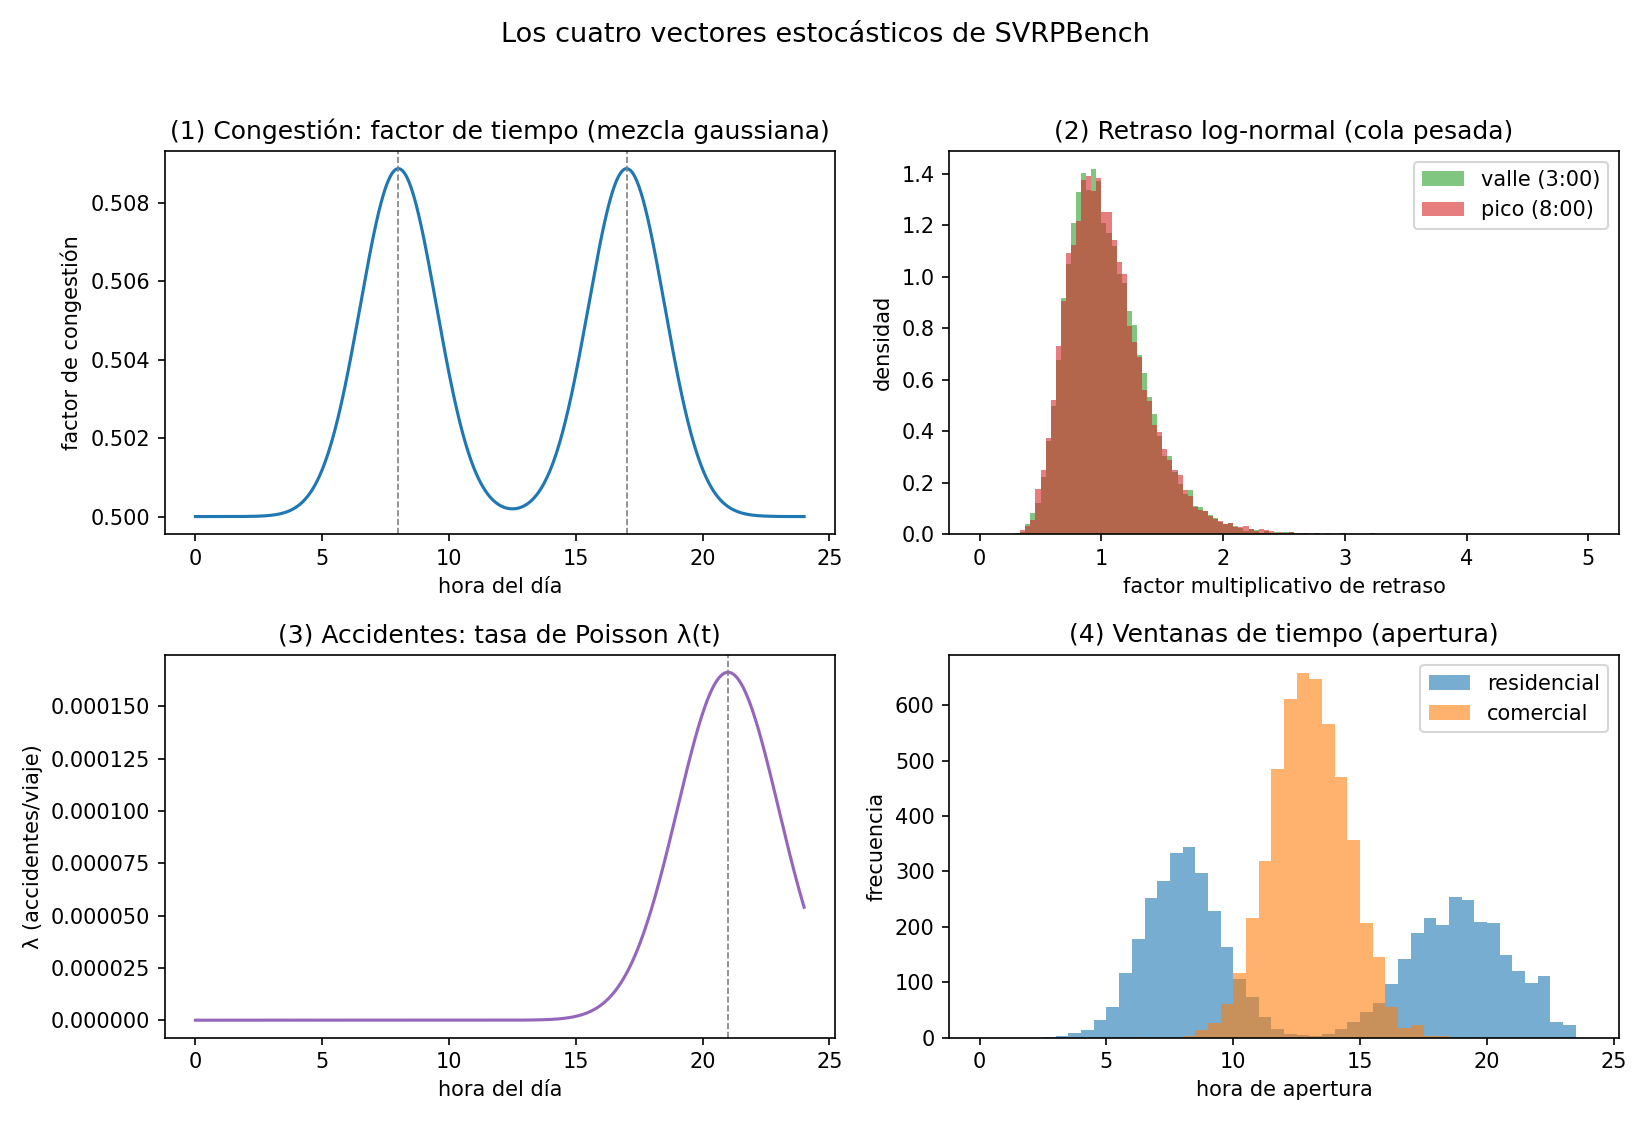
\includegraphics[width=0.95\textwidth]{stochastic_model.png}
  \caption{Los cuatro vectores estocásticos de SVRPBench. El panel~(2) muestra que el retraso
  log-normal tiene cola pesada; el panel~(3), que los accidentes son rarísimos
  ($\lambda\!\approx\!1.6\times10^{-4}$): de ahí que, a la tasa oficial, la variabilidad del
  costo sea pequeña.}
  \label{fig:stoch}
\end{figure}

% =====================================================================
\section{Marco de evaluación}
\label{sec:eval}

Todas las soluciones (rutas a priori) se puntúan con un \textbf{evaluador estocástico
compartido}. Sus pilares:

\paragraph{Common Random Numbers (CRN).} Por cada realización $r$ se pre-muestrea un escenario
$\xi_r$ (ruido log-normal y accidentes por arco $\times$ \emph{bucket} horario)
\emph{independiente de la ruta} y determinista en $(\text{seed},r)$. Así, dos métodos
cualesquiera sobre la misma instancia ven \emph{exactamente} el mismo $\xi_r$: la comparación
es de varianza reducida y estadísticamente válida.

\paragraph{Métricas.} Por instancia se reportan: costo esperado de viaje $E[c]$; costo total
con recurso $E[c+Q]$; \textbf{CVaR}$_\alpha(c+Q)$ (media del peor $(1-\alpha)$ de los
escenarios, medida sensible al riesgo de cola, $\alpha=0.95$); \textbf{tasa de factibilidad}
(fracción de realizaciones sin violaciones); tasa de violación CVR (\%); robustez
(desviación estándar de $c$); número de vehículos; y tiempo de cómputo.

\paragraph{Homologación de condiciones.} Para garantizar igualdad de condiciones, el
\emph{runner} aplica una \textbf{re-puntuación unificada}: tras resolver, las rutas de cada
método se vuelven a puntuar con el mismo evaluador y los mismos parámetros
(Tabla~\ref{tab:cond}), independientemente de la puntuación interna del solver. El costo de
flota se internaliza de forma uniforme mediante un costo fijo por vehículo
($\code{--vehicle-cost}$), evitando premiar la ``factibilidad a cambio de más vehículos''.

\begin{table}[h]
  \centering
  \caption{Condiciones experimentales homologadas (idénticas para los cuatro paradigmas).}
  \label{tab:cond}
  \begin{tabular}{ll}
    \toprule
    \textbf{Condición} & \textbf{Valor (igual para todos)}\\
    \midrule
    Instancias & misma lista; mismo \code{seed} por instancia\\
    Escenarios $\xi$ & CRN: \code{seed = metadata.seed} $\Rightarrow$ $\xi$ idéntico\\
    Realizaciones Monte Carlo & 200\\
    Modo de capacidad & \code{binding} (capacidad activa)\\
    Tasa de accidentes & $\times 1$ (fiel a SVRPBench)\\
    Penalización de recurso & $\text{late\_penalty}=1$ por minuto de retraso\\
    Costo de flota & uniforme (\code{--vehicle-cost}; $0=$ sólo viaje)\\
    \bottomrule
  \end{tabular}
\end{table}

\noindent\textbf{No homologable} (inherente a cada paradigma, declarado): (i)~el objetivo que
optimiza cada método difiere (los exactos/NCO minimizan el tiempo de viaje nominal $\tau$; las
metaheurísticas su costo muestreado; todos se \emph{evalúan} igual); (ii)~las NCO tienen un
\textbf{costo de entrenamiento} amortizado fuera del \code{runtime} de inferencia.

% =====================================================================
\section{Los cuatro paradigmas (métodos)}
\label{sec:metodos}

\subsection{Paradigma 1 --- Métodos Exactos (Branch \& Cut)}
Solver \code{exact-bc} (CVRP) y \code{exact-bc-tw} (CVRPTW). Formulación de flujo no dirigida
de dos índices resuelta con Gurobi y \textbf{branch-and-cut} genuino: desigualdades de
capacidad redondeada / eliminación de subtours (RCI/DFJ) separadas como \emph{lazy
constraints}. El objetivo minimiza el tiempo de viaje \emph{nominal} $\tau_{ij}=d_{ij}+$
retraso de congestión determinista. Garantiza el óptimo en instancias pequeñas pero su
intratabilidad se manifiesta al crecer $n$ (Fig.~\ref{fig:conv}). Incluye una aserción de
factibilidad post-solve (cada ruta respeta la capacidad, cada cliente se sirve una vez) como
red de seguridad.

\begin{figure}[h]
  \centering
  
\includegraphics[width=0.6\textwidth]{exact-bc_n50_i0_convergence.png}
  \caption{Convergencia de Branch \& Cut en $n=50$: el incumbente (rojo) mejora rápido pero la
  cota inferior (azul) se estanca; la brecha (gap) permanece amplia al límite de tiempo. Es la
  barrera de escalabilidad del paradigma exacto.}
  \label{fig:conv}
\end{figure}

\subsection{Paradigma 2 --- Metaheurísticas (ACO y Tabu)}
Solvers \code{aco} y \code{tabu}, que envuelven las implementaciones \emph{oficiales} de
SVRPBench (Ant System genuino con regla de transición $\tau^\alpha\eta^\beta$, evaporación y
depósito de feromona $Q/L$; Tabu Search con lista tabú y manejo de infactibilidad por
penalización), re-puntuadas con CRN. Son deterministas (semilla fija) con agregación
\emph{best-of-K} sobre varias semillas.

\subsection{Paradigma 3 --- NCO supervisado (Pointer Network)}
Solver \code{nco-sl}. Red de Apuntadores (codificador LSTM + atención puntero) entrenada de
forma \textbf{supervisada} (imitación con \emph{teacher forcing}) sobre rutas óptimas de un
\textbf{maestro configurable}: \code{nco-sl} imita a \code{exact-bc} (óptimo, ignora ventanas)
y \code{nco-sl-feas} imita a \code{aco} (factible). Hallazgo clave: la (in)factibilidad la
define el \emph{maestro}, no el paradigma. Inferencia en milisegundos. (No existe baseline de
NCO supervisado en SVRPBench; es implementación propia.)

\subsection{Paradigma 4 --- NCO por RL (POMO)}
Solver \code{nco-rl}. La \emph{misma} arquitectura del paradigma 3 entrenada por
\textbf{REINFORCE estilo POMO}: $N$ trayectorias desde nodos de inicio distintos y la media de
sus costos como \textbf{línea base compartida}; recompensa $=$ costo determinista, sin
etiquetas, con bonus de entropía. \emph{Declaración honesta}: se aplica el \emph{esquema} POMO
sobre una Pointer Network (LSTM), no sobre el \emph{Attention Model} transformer; es un proxy
competitivo a escala pequeña, no SOTA a gran escala.

% =====================================================================
\section{Resultados y discusión}
\label{sec:resultados}

Las Tablas~\ref{tab:n10} y~\ref{tab:n20} resumen la comparación homologada (5 instancias por
tamaño, 200 realizaciones, costo de flota $=0$). Las figuras~\ref{fig:bars},
\ref{fig:tradeoff} y~\ref{fig:runtime} la visualizan.

\begin{table}[h]
  \centering
  \caption{Resultados homologados, $n=10$ (promedios sobre 5 instancias).}
  \label{tab:n10}
  \begin{tabular}{lrrrrrr}
    \toprule
    Método (paradigma) & $E[c]$ & $E[c{+}Q]$ & CVaR & feas. & veh. & $t$ (s)\\
    \midrule
    \code{exact-bc} (1)    & \textbf{2173} & 3106 & 3106 & 0.00 & 3.0 & 0.01\\
    \code{nco-rl} (4)      & 2212 & 3457 & 3458 & 0.00 & 3.4 & 0.01\\
    \code{nco-sl} (3)      & 2292 & 3900 & 3901 & 0.00 & 3.4 & 0.00\\
    \code{aco} (2)         & 3066 & 3066 & 3066 & \textbf{1.00} & 5.8 & 0.21\\
    \code{nco-sl-feas} (3) & 3201 & 3946 & 3947 & 0.20 & 6.2 & 0.00\\
    \code{tabu} (2)        & 3419 & 3419 & 3419 & \textbf{1.00} & 6.0 & 0.69\\
    \bottomrule
  \end{tabular}
\end{table}

\begin{table}[h]
  \centering
  \caption{Resultados homologados, $n=20$ (promedios sobre 5 instancias).}
  \label{tab:n20}
  \begin{tabular}{lrrrrrr}
    \toprule
    Método (paradigma) & $E[c]$ & $E[c{+}Q]$ & CVaR & feas. & veh. & $t$ (s)\\
    \midrule
    \code{exact-bc} (1)    & \textbf{3356} & 5865 & 5866 & 0.00 & 4.0 & 0.10\\
    \code{nco-rl} (4)      & 3430 & 5652 & 5653 & 0.00 & 4.0 & 0.01\\
    \code{nco-sl} (3)      & 3991 & 5983 & 5983 & 0.00 & 4.8 & 0.00\\
    \code{aco} (2)         & 6951 & 6951 & 6952 & \textbf{1.00} & 11.6 & 0.65\\
    \code{tabu} (2)        & 7541 & 7541 & 7541 & \textbf{1.00} & 11.8 & 1.91\\
    \code{nco-sl-feas} (3) & 7766 & 8369 & 8370 & 0.20 & 15.2 & 0.01\\
    \bottomrule
  \end{tabular}
\end{table}

\begin{figure}[h]
  \centering
  
\includegraphics[width=0.99\textwidth]{comparison_metrics.png}
  \caption{Comparación por tamaño y método (6 solvers, 4 paradigmas). Paneles: costo esperado,
  costo total con recurso, factibilidad, CVaR y número de vehículos.}
  \label{fig:bars}
\end{figure}

\subsection{Hallazgo central: dos familias y un hueco}

La Figura~\ref{fig:tradeoff} es la síntesis del estudio. Emergen \textbf{dos familias}:
\begin{itemize}[nosep]
  \item \textbf{Costo-óptimos, frágiles ante ventanas} (esquina inferior-izquierda): exacto,
  \code{nco-rl}, \code{nco-sl}. Logran el menor $E[c]$ con pocos vehículos (3--5), pero su
  factibilidad es $0$ bajo la estocasticidad de las ventanas.
  \item \textbf{Factibles, costosos en flota} (esquina superior-derecha): \code{aco},
  \code{tabu}, \code{nco-sl-feas}. Alcanzan factibilidad $\approx 1$ pero usando $\sim 3\times$
  más vehículos y, por tanto, mucho mayor costo.
\end{itemize}
\textbf{Ningún método ocupa la esquina superior-izquierda} (bajo costo \emph{y} alta
factibilidad): ese es precisamente el hueco que la propuesta EHBG-FACS pretende cerrar.

\begin{figure}[h]
  \centering
  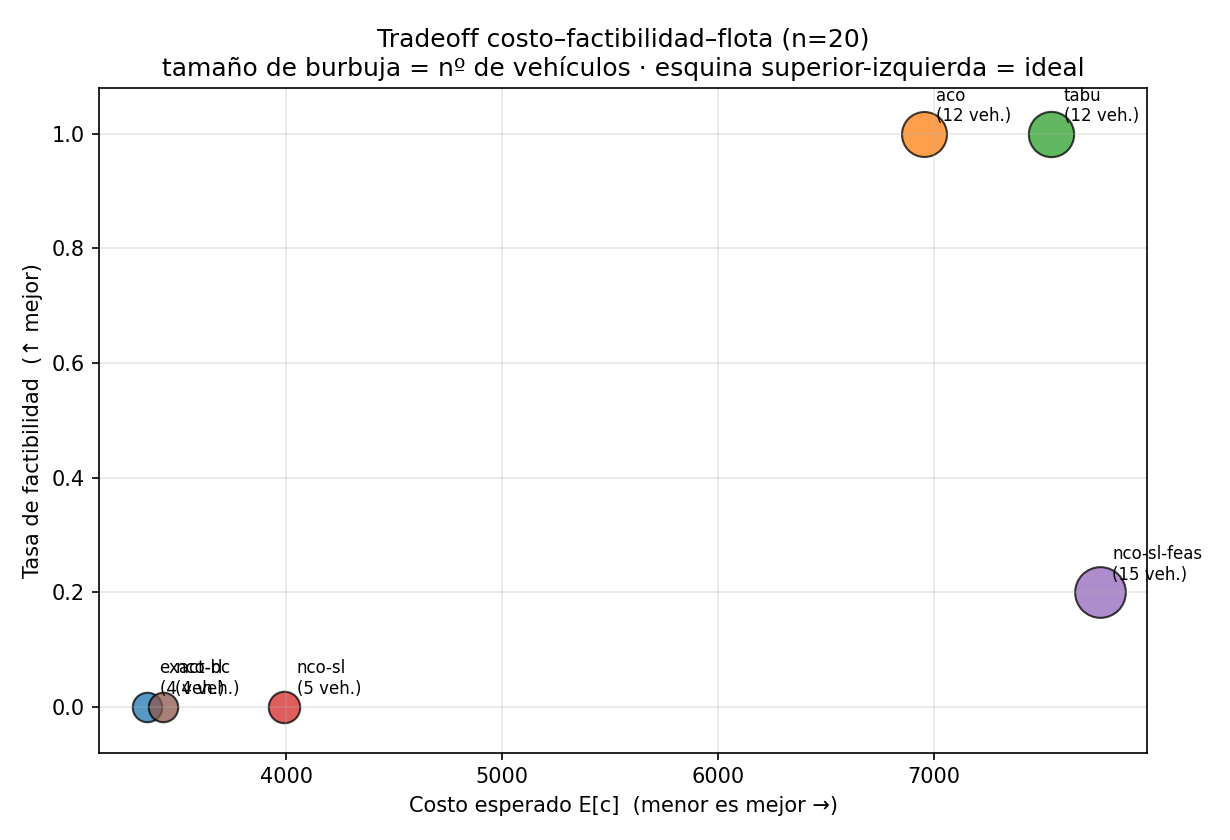
\includegraphics[width=0.78\textwidth]{tradeoff.png}
  \caption{Tradeoff costo--factibilidad--flota ($n=20$). El tamaño de la burbuja es el número
  de vehículos. La región ideal (arriba-izquierda) está vacía.}
  \label{fig:tradeoff}
\end{figure}

\subsection{Otros hallazgos}
\begin{itemize}[nosep]
  \item \textbf{RL $>$ supervisado.} Bien entrenado (excluyendo el log-prob del nodo forzado y
  con entropía), \code{nco-rl} (POMO) queda a $\sim$2.6\,\% del óptimo en $n=20$ y supera a
  \code{nco-sl} ($\sim$19\,\%) --- coherente con la literatura (el RL se consolidó como motor
  dominante en NCO).
  \item \textbf{Inferencia neuronal en milisegundos} (Fig.~\ref{fig:runtime}): las NCO
  producen su solución $\sim 10$--$200\times$ más rápido que las metaheurísticas, y sin
  resolver un MIP. El costo de entrenamiento es único y amortizable.
  \item \textbf{La estocasticidad de SVRPBench (a la tasa oficial) apenas mueve el costo}: la
  robustez $\sigma$ es pequeña y CVaR$\approx$media, porque los accidentes son rarísimos
  (Fig.~\ref{fig:stoch}-3). La señal discriminante principal es la \emph{factibilidad/recurso}
  ante ventanas, no la varianza del costo.
\end{itemize}

\begin{figure}[h]
  \centering
  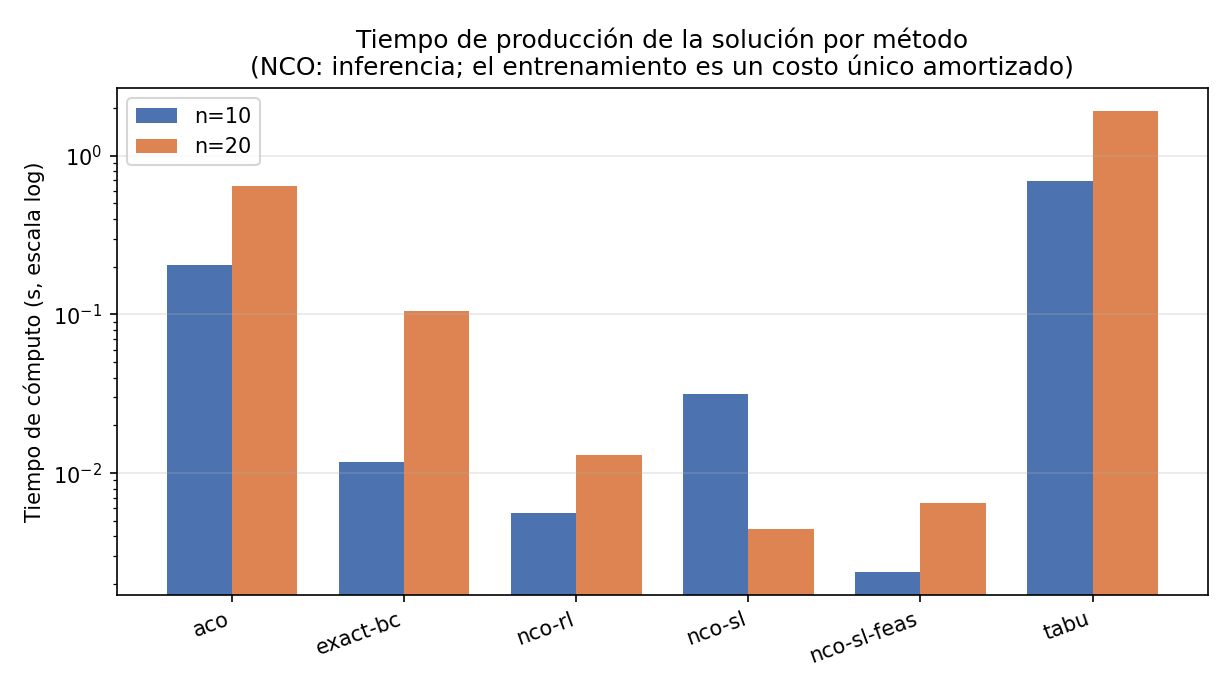
\includegraphics[width=0.74\textwidth]{runtime.png}
  \caption{Tiempo de producción de la solución (escala log). Las NCO infieren en milisegundos;
  el exacto crece con $n$; las metaheurísticas son las más lentas a esta escala.}
  \label{fig:runtime}
\end{figure}

% =====================================================================
\section{Conclusiones y trabajo futuro}
\label{sec:conclusiones}

Se implementaron y compararon, bajo condiciones homologadas y verificadas, los cuatro
paradigmas base. La comparación es justa (mismas instancias, escenarios, parámetros y
re-puntuación unificada) y los métodos son fieles a la literatura (con la salvedad declarada de
que el paradigma~4 usa la arquitectura pointer-net y no el transformer AM). El resultado
central —dos familias separadas, sin ningún método en la región ideal— motiva directamente la
hipótesis de la tesis: un marco híbrido GFlowNet de balance híbrido + colonia de hormigas
(EHBG-FACS) que busque \emph{simultáneamente} bajo costo y alta factibilidad.

\noindent\textbf{Pendiente para la comparación final (paradigma 5):} (i)~elevar a $\geq 30$
instancias por tamaño y aplicar ANOVA / Wilcoxon ($\alpha=0.05$); (ii)~fortalecer el baseline
POMO con codificador AM-transformer / RL4CO para escalas mayores; (iii)~escalar a $n\in[50,300]$
con licencia académica de Gurobi para la cota exacta.

% =====================================================================
\section{Diccionario (glosario)}
\label{sec:glosario}

\subsection*{Acrónimos}
\begin{longtable}{p{2.6cm}p{12.5cm}}
  \toprule
  \textbf{Acrónimo} & \textbf{Significado}\\
  \midrule
  \endhead
  VRP & Vehicle Routing Problem (Problema de Enrutamiento de Vehículos).\\
  CVRP & Capacitated VRP (con restricción de capacidad).\\
  TWCVRP & Time-Window CVRP (con ventanas de tiempo).\\
  SVRP & Stochastic VRP (estocástico).\\
  SVRPBench & Benchmark estocástico de alta fidelidad para SVRP.\\
  NCO & Neural Combinatorial Optimization (Optimización Combinatoria Neuronal).\\
  RL & Reinforcement Learning (Aprendizaje por Refuerzo).\\
  ACO & Ant Colony Optimization (Optimización por Colonia de Hormigas).\\
  B\&C & Branch \& Cut (ramificación y corte).\\
  MIP & Mixed-Integer Program (programación entera mixta).\\
  RCI/DFJ & Rounded Capacity Inequalities / Dantzig--Fulkerson--Johnson (cortes de capacidad y subtour).\\
  MTZ & Miller--Tucker--Zemlin (variables de tiempo/orden para eliminar subtours).\\
  POMO & Policy Optimization with Multiple Optima (RL con múltiples inicios y línea base compartida).\\
  AM & Attention Model (modelo de atención tipo transformer para ruteo).\\
  GFlowNet & Generative Flow Network (Red de Flujo Generativo).\\
  HBG & Hybrid-Balance GFlowNet.\\
  GFACS & Generative Flow Ant Colony Sampler.\\
  EHBG-FACS & Epistemic HBG-FACS (la propuesta de la tesis).\\
  ENN & Epistemic Neural Network (Red Neuronal Epistémica).\\
  CVaR & Conditional Value-at-Risk (Valor en Riesgo Condicional).\\
  CRN & Common Random Numbers (números aleatorios comunes).\\
  CRA/CVR & Constraint Violation Rate (tasa de violación de restricciones).\\
  REINFORCE & Algoritmo de gradiente de política de Monte Carlo.\\
  CE & Cross-Entropy (entropía cruzada, pérdida supervisada).\\
  \bottomrule
\end{longtable}

\subsection*{Variables y símbolos}
\begin{longtable}{p{2.6cm}p{12.5cm}}
  \toprule
  \textbf{Símbolo} & \textbf{Significado}\\
  \midrule
  \endhead
  $n$ & Número de clientes de la instancia (más el depósito = $n{+}1$ nodos).\\
  $\xi$ / $\xi_r$ & Escenario estocástico (realización $r$): congestión, retrasos, accidentes.\\
  $c(\text{ruta})$ & Costo de viaje (tiempo) de la ruta a priori.\\
  $Q(\text{ruta},\xi)$ & Costo de recurso de 2ª etapa (penalización por retraso al violar ventanas).\\
  $E[c]$ & Costo esperado de viaje (media Monte Carlo).\\
  $E[c{+}Q]$ & Costo total esperado con recurso.\\
  $\text{CVaR}_\alpha$ & Media del peor $(1{-}\alpha)$ de los costos ($\alpha=0.95$).\\
  $\tau_{ij}$ & Tiempo de viaje \emph{nominal} de $i$ a $j$ (distancia + congestión determinista a hora $t^\ast$).\\
  $d_{ij}$ & Distancia euclidiana entera entre $i$ y $j$.\\
  $\text{cap}$, $K$ & Capacidad del vehículo y número de vehículos/rutas.\\
  $\text{tf}(t)$ & Factor de congestión dependiente de la hora del día $t\in[0,1440)$ min.\\
  $\lambda(t)$ & Tasa del proceso de Poisson de accidentes.\\
  $x_{ij}$ / $y_{e}$ & Variables de arco dirigido / arista no dirigida del MIP.\\
  $P_F, P_B, F_\theta$ & Políticas de avance/retroceso y flujo de estado de la GFlowNet.\\
  $\alpha,\beta,\rho,Q$ & ACO: importancia de feromona, de heurística, evaporación, constante de depósito.\\
  feas. & Tasa de factibilidad $\in[0,1]$.\\
  $\sigma$ (robustez) & Desviación estándar de $c$ entre realizaciones.\\
  \bottomrule
\end{longtable}

\subsection*{Métodos / solvers implementados}
\begin{longtable}{p{2.7cm}p{2.0cm}p{9.6cm}}
  \toprule
  \textbf{Solver} & \textbf{Paradigma} & \textbf{Descripción}\\
  \midrule
  \endhead
  \code{exact-bc} & 1 Exacto & CVRP por Branch \& Cut (Gurobi), formulación no dirigida + cortes RCI lazy.\\
  \code{exact-bc-tw} & 1 Exacto & CVRPTW dirigido con MTZ y ventanas \emph{soft}.\\
  \code{aco} & 2 Metaheur. & Ant System oficial (NN+2opt + feromona), re-puntuado con CRN.\\
  \code{tabu} & 2 Metaheur. & Tabu Search oficial (lista tabú + reparación), re-puntuado con CRN.\\
  \code{nco-sl} & 3 NCO sup. & Pointer Network supervisada que imita a \code{exact-bc}.\\
  \code{nco-sl-feas} & 3 NCO sup. & Variante que imita a \code{aco} (maestro factible).\\
  \code{nco-rl} & 4 NCO RL & Pointer Network entrenada por REINFORCE estilo POMO (costo determinista).\\
  \bottomrule
\end{longtable}

\subsection*{Software y entorno}
Python 3.13 sobre Apple~M1 (8\,GB); Gurobi (licencia restringida); PyTorch (CPU) para las NCO;
\code{scikit-learn}/\code{Pillow} para el generador oficial. El paquete \code{vrp\_bench} de
SVRPBench se usa vía \code{PYTHONPATH}. El harness reproducible vive en \code{experiments/svrp/}.

\end{document}
